\documentclass[11pt]{article}
\usepackage[utf8]{inputenc}
\usepackage{fullpage}
\usepackage{amsmath}
\usepackage{mathtools}
\usepackage{amssymb}
\usepackage{listings}
\usepackage{color}
\usepackage{booktabs}
\usepackage{multirow}
\usepackage{siunitx}
\usepackage{pdflscape}
\usepackage{pgfplots}
\usepackage{enumitem}

\title{Programming Exercise for Mathematical Programming 186.835}
\author{Benjamin Schwendinger \\
e1225371}


\sisetup{round-mode=places,round-precision=3}

\begin{document}

\maketitle
\section{k-Node Minimum Spanning Tree (k-MST) Problem}
\textbf{Given:}
\begin{itemize}
\item graph $G = (V,E,w)$
\item edge weights $w(e) \in \mathbb{R_0^+}, \forall e \in E$
\item integer $0 \leq k \leq |V|$
\end{itemize}
\textbf{Goal:} Find a minimum weight tree, spanning exactly k nodes.
\\ \\
I use a directed graph to model the problem. Hence for each edge in $E$, I use two directed arcs instead. Moreover, the weight of each arc is the same as the corresponding weight of the undirected graph. Furthermore a root node (I call it 0) and edges from 0 to each other node with weight 0 are added. I write the set of neighbors of a vertex $v$ as $N(v)$.

\section{Formulations}
\subsection{Variables:}
\subsubsection{Binary variables:}
\[
x_e = 
\begin{cases}
1 & \text{if edge $e$ is in the tree} \\
0 & \text{otherwise} 
\end{cases}
\]

\[
y_a = 
\begin{cases}
1 & \text{if arc $a$ is in the tree} \\
0 & \text{otherwise} 
\end{cases}
\]

\[
z_v = 
\begin{cases}
1 & \text{if vertex $v$ is in the tree} \\
0 & \text{otherwise} 
\end{cases}
\]

\subsubsection{Integer variables:}
order variables $u_i$ are used to indicate the order in which the nodes are explored (start and end node is 0) \\ 
flow variables $0 \leq f_{ij} \leq n-1$; amount of flow on arc $(i,j) \in A$

\subsection{MTZ}
\begin{subequations}
\begin{align}
 &\min_{e \in E} c_e x_e&  \\
\text{subject to }  &\sum_{a \in A} y_a = k+1& \\
 &\sum_{v \in V} z_v = k+1  \\
 &\sum_{j \in N(i)} y_{ij} \leq 1  & \forall v \in V \\
 & \sum_{i \in N(0)}y_{i0} = \sum_{i \in N(0)} y_{0i}  = 1  \\
 & y_{ij} \leq z_i, z_j & \forall i,j \in V \\
 & y_{ij} + y_{ji} = x_e & \forall e=\{i,j\}, e \in E \\
 & u_i + y_{ij} \leq u_j + (n-2)(1-y_{ij}) &\forall i,j \in V \setminus \{0\}, i \neq j \\
 & 1 \leq u_i \leq n-1 & \forall i \in V \setminus \{0\} \\
 & z_v \in \{0,1\} & \forall v \in V \\
 & x_e \in \{0,1\} & \forall e \in E \\
 & y_a \in \{0,1\} & \forall a \in A 
\end{align}
\end{subequations}

\subsection{SCF}
\begin{subequations}
\begin{align}
 &\min_{e \in E} c_e x_e&  \\
\text{subject to }  &\sum_{a \in A} y_a = k+1& \\
 &\sum_{v \in V} z_v = k+1  \\
 &\sum_{j \in N(i)} y_{ij} \leq 1  & \forall v \in V \\
 & \sum_{i \in N(0)}y_{i0} = \sum_{i \in N(0)} y_{0i}  = 1  \\
 & y_{ij} \leq z_i, z_j & \forall i,j \in V \\
 & y_{ij} + y_{ji} = x_e & \forall e=\{i,j\}, e \in E \\
 & \sum_{j \in N(i)} f_{ij} - \sum_{j \in N(i)} f_{ji} = y_i & \forall i \in V \setminus{\{0\}}\\	
 & 0 \leq f_{ij} \leq (n-1) y_{ij} & \forall (i,j) \in A \\
 & z_v \in \{0,1\} & \forall v \in V \\
 & x_e \in \{0,1\} & \forall e \in E \\
 & y_a \in \{0,1\} & \forall a \in A 
\end{align}
\end{subequations}
The objective is modelled by Equation $(a)$ which states the weight of the found tree has to be minimal. \\
The constraints $(b)$ to $(f)$ are the same for both formulations.
\begin{enumerate}[label=(\alph*)]
\setcounter{enumi}{1}
\item Our found directed graphs has to have $k+1$ arcs. Hence I get a tree on by deleting the arcs from and to 0.
\item Our found tree has to have $k+1$ nodes. This is true, since I am searching for a tree on $k$ for graph without our added root node.
\item The number of ingoing arcs to every node is less or equal 1. This enforces that the found graph is a forest.
\item The number of ingoing and outgoing arcs from 0 is 1. This enforces that really $k-1$ edges of the input graph are used and not only our added zero weight edges from and to 0.
\item An arc can only be in the tree if both ends of it are in the tree.
\item An edge is in the graph if one and at most one of the corresponding arcs is in the directed graph.
\end{enumerate}
The constraints $(1h)$ to $(1i)$ model the MTZ constraints. \\
The constraints $(2h)$ to $(2i)$ model the SCF constraints. Here a node only consumes one if it is in the tree. \\
The constraints $j$ to $k$ set the domains of my binary variables.
\section{Computational Results}
The implementations are done in Python and I use Gurobi 8 to solve our ILP approach.
All tests were performed on a single core of an 
Intel Xeon E5540 processor with 2.53 GHz
using at most 3GB RAM.
\\ \\
According to Table \ref{table:results} and Figure \ref{plot:nodes} I see that MTZ has to explore more nodes for bigger $k$ ($k \geq 100$). The running times show similiar results according to Table \ref{table:results} and Figure \ref{plot:runtimes}, although it seems that MTZ is favorable for smaller $k$. This is probably due to the high number of nodes which are explored for bigger $k$. Moreover, we see that all optimal values are reached with both developed formulations.
%\begin{landscape}
\begin{table}
  \begin{tabular}{SSSSSSSS}
    \toprule
    \multicolumn{2}{c}{Inputs} &
    \multicolumn{3}{c}{MTZ} &
    \multicolumn{3}{c}{SCF} \\
    {Instance} & {k} & {Objective} & {Nodes explored} & {Time(s)} & {Objective } & {Nodes explored} & {Time(s)} \\
    \midrule
1 & 2   & 46    & 0      & 0.07802057266235352 & 46    & 0     & 0.03599429130554199 \\
1 & 5   & 477   & 0      & 0.03252410888671875 & 477   & 16    & 0.04291081428527832 \\
2 & 4   & 373   & 19     & 0.12757420539855957 & 373   & 89    & 0.11484718322753906 \\
2 & 10  & 1390  & 42     & 0.0865168571472168  & 1390  & 0     & 0.15539121627807617 \\
3 & 10  & 725   & 258    & 0.22100543975830078 & 725   & 459   & 0.4177205562591553  \\
3 & 25  & 3074  & 3687   & 0.5808014869689941  & 3074  & 72    & 0.4948270320892334  \\
4 & 14  & 909   & 1465   & 0.4982266426086426  & 909   & 1257  & 1.468893051147461   \\
4 & 35  & 3292  & 1859   & 1.6151392459869385  & 3292  & 2750  & 1.5517733097076416  \\
5 & 20  & 1235  & 1669   & 1.644547462463379   & 1235  & 1767  & 1.9977211952209473  \\
5 & 50  & 4898  & 3348   & 1.8911528587341309  & 4898  & 4709  & 3.432373523712158   \\
6 & 40  & 2068  & 17374  & 14.874151229858398  & 2068  & 17679 & 45.048290729522705  \\
6 & 100 & 6705  & 19768  & 19.76146149635315   & 6705  & 7934  & 27.087477684020996  \\
7 & 60  & 1335  & 1631   & 32.16856336593628   & 1335  & 1743  & 56.404672622680664  \\
7 & 150 & 4534  & 3337   & 33.05476498603821   & 4534  & 4548  & 108.3318018913269   \\
8 & 80  & 1620  & 3138   & 36.99395775794983   & 1620  & 1805  & 115.92533326148987  \\
8 & 200 & 5787  & 146821 & 414.95961332321167  & 5787  & 3872  & 193.72209477424622  \\
 \bottomrule
  \end{tabular}
\caption{Result table for different formulations}
\label{table:results}
\end{table}
%\end{landscape}

\begin{figure}
\begin{minipage}{0.4\textwidth}
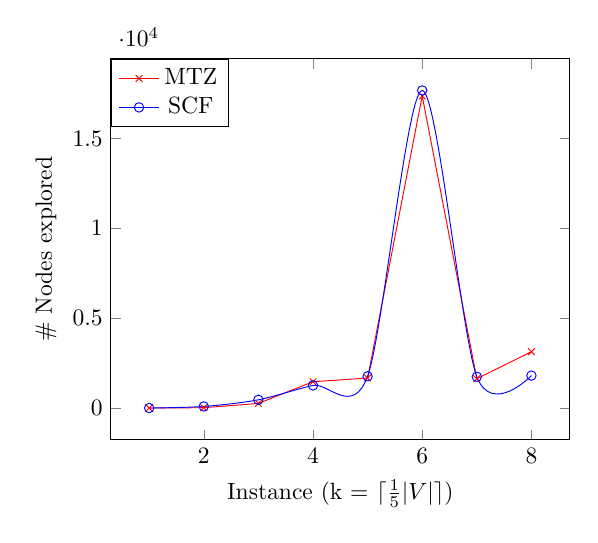
\begin{tikzpicture}[scale=0.85] 
\begin{axis}[ xlabel={Instance (k = $\lceil \frac{1}{5} |V| \rceil$)}, ylabel=\# Nodes explored=log, legend style={at={(0,1)},anchor=north west}] 
\addplot[color=red,mark=x] coordinates {(1,0.0) (2,19.0) (3,258.0) (4,1465.0) (5,1669.0) (6,17374.0) (7,1631.0) (8,3138.0)};
\addplot[smooth,color=blue,mark=o] coordinates {(1,0.0) (2,89.0) (3,459.0) (4,1257.0) (5,1767.0) (6,17679.0) (7,1743.0) (8,1805.0)};

\legend{MTZ, SCF}
\end{axis} 
\end{tikzpicture}
\end{minipage}
\hfill
\begin{minipage}{0.4\textwidth}
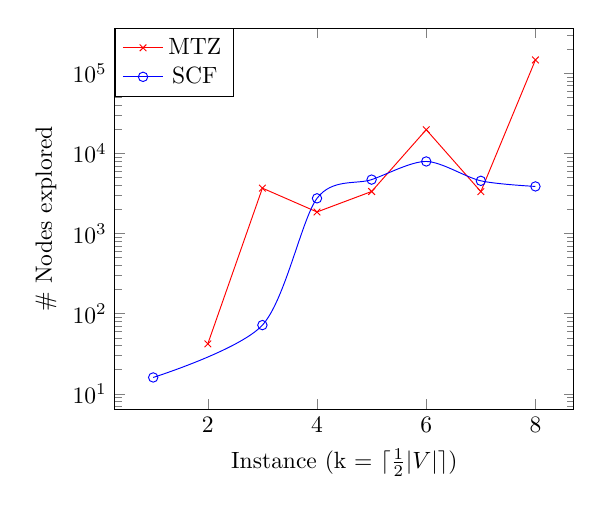
\begin{tikzpicture}[scale=0.85] 
\begin{axis}[ xlabel={Instance (k = $\lceil \frac{1}{2} |V| \rceil$)}, ylabel=\# Nodes explored, ymode=log, legend style={at={(0,1)},anchor=north west}] 
\addplot[color=red,mark=x] coordinates {(1,0.0) (2,42.0) (3,3687.0) (4,1859.0) (5,3348.0) (6,19768.0) (7,3337.0) (8,146821.0)};
\addplot[smooth,color=blue,mark=o] coordinates {(1,16.0) (2,0.0) (3,72.0) (4,2750.0) (5,4709.0) (6,7934.0) (7,4548.0) (8,3872.0)};


\legend{MTZ, SCF}
\end{axis} 
\end{tikzpicture}
\end{minipage}
\caption{Number of explored nodes for different formulations} \label{plot:nodes}
\end{figure}

\begin{figure}
\begin{minipage}{0.4\textwidth}
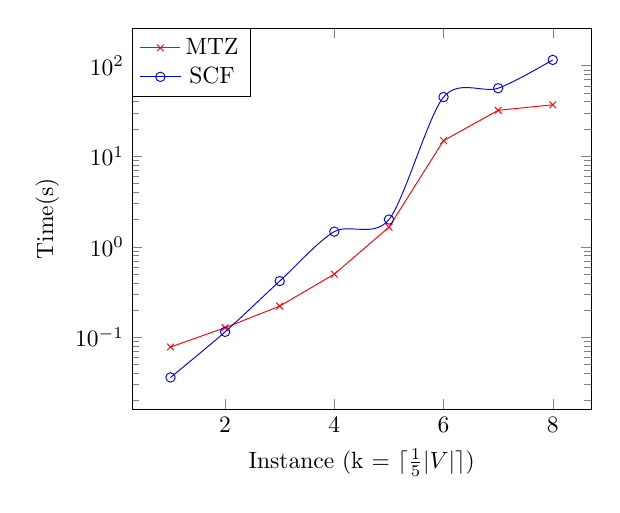
\begin{tikzpicture}[scale=0.85] 
\begin{axis}[ xlabel={Instance (k = $\lceil \frac{1}{5} |V| \rceil$)}, ylabel=Time(s), ymode=log, legend style={at={(0,1)},anchor=north west}] 
\addplot[color=red,mark=x] coordinates {(1,0.07802057266235352) (2,0.12757420539855957) (3,0.22100543975830078) (4,0.4982266426086426) (5,1.644547462463379) (6,14.874151229858398) (7,32.16856336593628) (8,36.99395775794983)}; 
\addplot[smooth,color=blue,mark=o] coordinates {(1,0.03599429130554199) (2,0.11484718322753906) (3,0.4177205562591553) (4,1.468893051147461) (5,1.9977211952209473) (6,45.048290729522705) (7,56.404672622680664) (8,115.92533326148987)};

\legend{MTZ, SCF}
\end{axis} 
\end{tikzpicture}
\end{minipage}
\hfill
\begin{minipage}{0.4\textwidth}
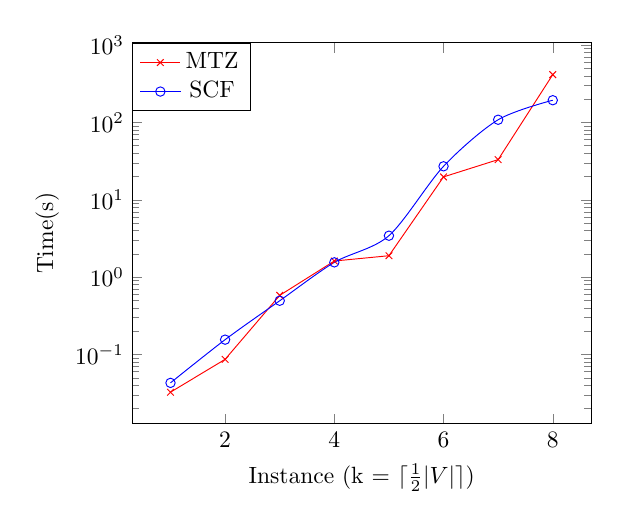
\begin{tikzpicture}[scale=0.85] 
\begin{axis}[ xlabel={Instance (k = $\lceil \frac{1}{2} |V| \rceil$)}, ylabel=Time(s), ymode=log, legend style={at={(0,1)},anchor=north west}] 
 \addplot[color=red,mark=x] coordinates {(1,0.03252410888671875) (2,0.0865168571472168) (3,0.5808014869689941) (4,1.6151392459869385) (5,1.8911528587341309) (6,19.76146149635315) (7,33.05476498603821) (8,414.95961332321167)};
 \addplot[smooth,color=blue,mark=o] coordinates {(1,0.04291081428527832) (2,0.15539121627807617) (3,0.4948270320892334) (4,1.5517733097076416) (5,3.432373523712158) (6,27.087477684020996) (7,108.3318018913269) (8,193.72209477424622)};

\legend{MTZ, SCF}
\end{axis} 
\end{tikzpicture}
\end{minipage}
\caption{Running times for different formulations} \label{plot:runtimes}
\end{figure}


\end{document}
